% !TeX encoding = UTF-8
% !TeX spellcheck = es_ES
% !TeX root = CBus.tex
%!TEX root=CBus.tex
CBus\sidenote{Usando CAN} ha sido pensado para seguir lo más fielmente posible una topologia de Bus y en los extremos una resistencia de \SI{120}{\ohm}.

\begin{figure}[H]
    \centering
    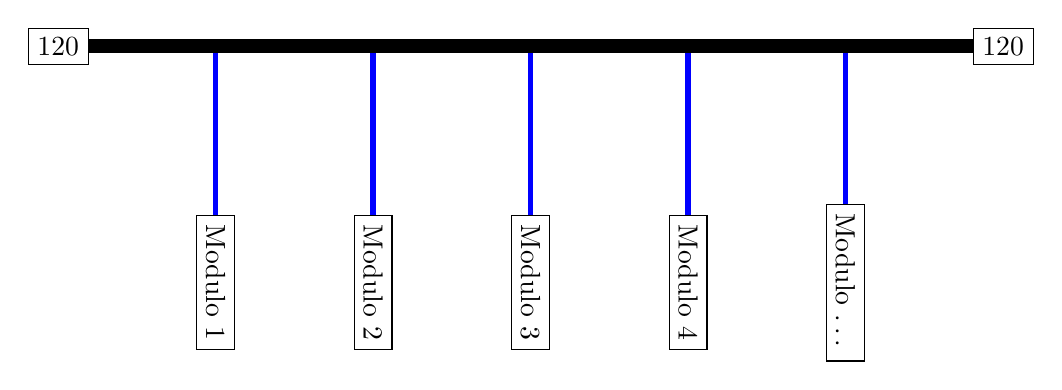
\begin{tikzpicture}
        %\draw [very thin, green]  (-6,-3) grid (6,3);
        \node at (-6,3) [rectangle,draw,align=left] (ps) {\SI{120}{\ohm}};
        \node at (6,3) [rectangle,draw,align=left] (ns) {\SI{120}{\ohm}};
        
        \node at (-4,0) [rectangle,draw,align=left,rotate=-90] (d1) {Modulo 1};
        \node at (-2,0) [rectangle,draw,align=left ,rotate=-90] (d2) {Modulo 2};
        \node at (0,0) [rectangle,draw,align=left ,rotate=-90] (d3) {Modulo 3};
        \node at (2,0) [rectangle,draw,align=left ,rotate=-90] (d4) {Modulo 4};
        \node at (4,0) [rectangle,draw,align=left ,rotate=-90] (d5) {Modulo \dots};

        \draw [line width=2, blue] (-4,3) --(d1.west);
        \draw [line width=2, blue] (-2,3) --(d2.west);
        \draw [line width=2, blue] (0,3) --(d3.west);
        \draw [line width=2, blue] (2,3) --(d4.west);
        \draw [line width=2, blue] (4,3) --(d5.west);

        \draw [line width=5] (ps.east) -- (ns.west);
    \end{tikzpicture}
    \caption{Topologia Bus}
    \label{fig:BusPuro}
\end{figure}
 
Pero a su vez permite algunas ramificaciones siempre y cuando la resitencia entre los conductores diferenciales sea aproximadamente \SI{60}{\ohm}. Ya que todos los modulos estaran conectados en paralelo a los 4 conductores.

Ademas CBUS, en general, permite utilizar otros sistemas de transporte de la informacion como puede ser
TCP, UDP, MQTT,\dots Pudiendo haber multiples Buses y segmentos unidos formando una red mayor.

\subsection{Red}
Recordemos que el objetivo de CBUS es poder controlar una maqueta de tren de forma digital. Es decir desde un
panel de mandos enviar señales para que suceda un cambio en la maqueta, o al reves, o ante un evento en la maqueta
\sidenote{Cortos, ocupacion por un tren,\dots} se actualice nuestro panel de control.

El panel de control puede ser fisico, (con lucecitas y botones) o bien puede ser una pantalla de un programa como JMRI
\sidenote{JMRI o similar, usaremos JMRI por preferencias del autor}

El caso minimo de uso CBus tendra un bus CAN con unos pocos modulos, partiendo el cable donde sea  necesario
y como mucho un CanUSB o CBusServer para conectar con JMRI. Vease \ref{fig:BusPuro}.
El caso más complejo requeria de uno o varios CBusServer cada uno conectado a uno o varios Buses CAN.
El/los CBusServer/es se comunicarian mediante TCP\sidenote{Wifi, Ethernet,\dots} entre si y distribuyendo asi los 
eventos entre todos los buses CAN.

Este ultimo caso lo podemos representar con dos buses CAN donde "Modulo 2" seria el CBusServer y
JMRI se conecta a traves de Wifi o un CanUSB.

\begin{figure}[H]
    \centering
    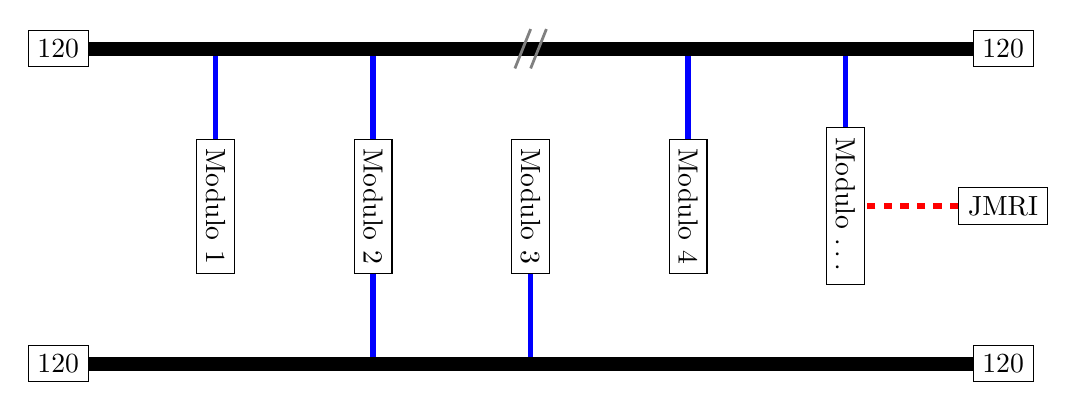
\begin{tikzpicture}
        %\draw [very thin, green]  (-6,-3) grid (6,3);
        \node at (-6,2) [rectangle,draw,align=left] (ps) {\SI{120}{\ohm}};
        \node at (6,2) [rectangle,draw,align=left] (ns) {\SI{120}{\ohm}};
        
        \node at (-6,-2) [rectangle,draw,align=left] (ps2) {\SI{120}{\ohm}};
        \node at (6,-2) [rectangle,draw,align=left] (ns2) {\SI{120}{\ohm}};

        \node at (-4,0) [rectangle,draw,align=left,rotate=-90] (d1) {Modulo 1};
        \node at (-2,0) [rectangle,draw,align=left ,rotate=-90] (d2) {Modulo 2};
        \node at (0,0) [rectangle,draw,align=left ,rotate=-90] (d3) {Modulo 3};
        \node at (2,0) [rectangle,draw,align=left ,rotate=-90] (d4) {Modulo 4};
        \node at (4,0) [rectangle,draw,align=left ,rotate=-90] (d5) {Modulo \dots};
        \node at (6,0) [rectangle,draw,align=left] (jmri) {JMRI};

        \draw [line width=2, blue] (-4,2) --(d1.west);
        \draw [line width=2, blue] (-2,2) --(d2.west);
        \draw [line width=2, blue] (-2,-2) --(d2.east);
        \draw [line width=2, blue] (0,-2) --(d3.east);
        \draw [line width=2, blue] (2,2) --(d4.west);
        \draw [line width=2, blue] (4,2) --(d5.west);

        \draw [line width=2, red, dashed] (jmri.west) --(d5.north);

        \draw [line width=5] (ps.east) -- (ns.west);
        \draw [line width=5] (ps2.east) -- (ns2.west);

        \draw [line width=1, gray] (-0.2,1.75)--(0,2.25) (0,1.75)--(0.2,2.25);


    \end{tikzpicture}
    \caption{Topologia Bus Ejemplo Red}
    \label{fig:RedEjemplo}
\end{figure}

La red CBUS es pues el conjunto de todos los dispositivos CBUS que se pueden comunicar entre si
usando el protocolo CBUS

\subsection{Segmento vs Bus vs Red vs CBusServer}
Sirva este apartado para aclarar y definir estos terminos. Puesto que esto son muy parecidos a una instalacion
TCP/IP.

Como ya se tiene la idea de lo que es la Red, empezaremos con el Bus. Siendo este el canal que permite
a todos los dispositivos conectados fisicamente al mismo. Hoy por Hoy solo hay dos tecnologias disponibles
\sidenote{segun este punto de vista}
\begin{itemize}
    \item \textbf{CAN Bus}: Utilizar un par diferencial CAN como comunicacion.
    \item \textbf{CBusServer}: Los dispositivos se conectan mediante una conexion TCP.
\end{itemize}